%mac
\begin{vidu}
Một người đẩy một thùng hàng, khối lượng $50\ kg$, trượt trên sàn nhà. Lực đẩy có phương nằm ngang với độ lớn là $180\ N$. Biết hệ số ma sát trượt giữa thùng hàng và sàn nhà là $0,25$. Lấy $g=9,8\ m/s^2$. Gia tốc của thùng hàng có độ lớn là bao nhiêu $m/s^2$?
\shortans[oly]{1,15}
\haidong{10}\loigiai{
\immini[thm]{\begin{itemize}
\item Thùng hàng chịu tác dụng của bốn lực: trọng lực $\vec P$, lực đẩy $\vec F$, phản lực $\vec N$ và lực ma sát trượt $\vec F_{ms}$ của sàn (Hình 20.1a).
\item Coi thùng hàng như một chất điểm (Hình 20.1b)
\item Áp dụng định luật 2 Newton cho chuyển động của vật theo hai trục Ox, Oy:
\begin{align*}
\begin{cases}
&Ox: F_x=F-F_{ms}=m.a_x=ma\quad (1)\\
&Oy: F_y=N-P=0\quad (2)
\end{cases}
\end{align*}
\item $F_{ms}=\mu N$
\item Giải hệ phương trình: \\
$N=mg=50.9,8=490\ N$\\
$F_{ms}=\mu.N=0,25.490=122,5\ N$\\
$a=\dfrac{F-F_{ms}}{m}=\dfrac{180-122,5}{50}=1,15\ m/s^2$.
\item Thùng hàng trượt với gia tốc $a=1,15\ m/s^2$ cùng chiều với trục Ox.
\end{itemize}}{\begin{tikzpicture}[scale=1,thick,>=stealth']
\tkzDefPoints{0/1/o}
\node  at  (0,0.32)  [shape=rectangle,draw=red,pattern=dots,minimum height=0.6cm,minimum width=1.4cm, rounded corners=1pt]  {};
\draw(-1.5,0)--(1.5,0);
\draw[very thick,blue,->](0.1,0)--++(90:1.8)node[right,black]{$\vec{N}$};
\draw[fill=white](0.1,0)circle(1.2pt);
\draw[very thick,blue,->](0,0.32)--++(-90:1.8)node[right,black]{$\vec{P}$};
\draw[fill=white](0,0.32)circle(1.2pt);
\draw[very thick,blue,->](-0.7,0)--++(180:1.2)node[above,black]{$\vec{F}_{ms}$};
\draw[fill=white](-0.7,0)circle(1.2pt);
\draw[very thick,blue,->](0.7,0.32)--++(0:2)node[above,black]{$\vec{F}$};
\draw[fill=white](0.7,0.32)circle(1.2pt);
\fill[pattern=north east lines](-1.5,0)--(1.5,0)--++(-90:0.1)--++(180:3);
\draw[->](2,1)node[below left]{$O$}--++(90:1.5)node[right]{$y$};
\draw[->](2,1)--++(0:2)node[above]{$x$};
\end{tikzpicture}}
}
\haidong{10} \end{vidu}

\begin{vidu}
\immini[thm]{Một người dùng dây buộc để kéo một thùng gỗ theo phương nằm ngang bằng một lực $\vec F$.  Khối lượng của thùng là $35\ kg$. Hệ số ma sát giữa sàn và đáy thùng là $0,3$. Lấy $g=9,8\ m/s^2$. Tính độ lớn của lực kéo trong hai trường hợp:	
\begin{itemize}
\item[a)] Thùng trượt với gia tốc $0,2\ m/s^2$.
\item[b)] Thùng trượt đều.
\end{itemize}}{
\includegraphics[width=0.5\linewidth]{images/20-2}}
\haidong{13}\loigiai{
\immini[thm]{\begin{itemize}
\item Thùng chịu tác dụng của bốn lực: trọng lực $\vec P=m.\vec g$, lực kéo $\vec F$, phản lực $\vec N$ và lực ma sát trượt $\vec F_{ms}$ của mặt sàn (Hình 20.3).
\item Coi thùng như một chất điểm (Hình 20.3b) và áp dụng định luật 2 Newton cho các lực thành phần theo các phương Ox, Oy.
\begin{align*}
\begin{cases}
&F_x=F-F_{ms}=m.a_x=m.a\quad (1)\\
&F_y=N-P=0\quad (2)
\end{cases}
\end{align*}
\item $F_{ms}=\mu . N$
\item Giải hệ phương trình: \\
Từ $(2)\Rightarrow N=m.g$\\
Suy ra: $F_{ms}=\mu.N=\mu.mg$
\item Thay vào $(1)$ ta được: \\
$F=m.a+\mu mg$\\
$F=m(a+\mu g)$
\end{itemize}
\begin{itemize}
\item[a)] Thùng trượt với gia tốc $a=0,2\ m/s^2$\\
$F=m(a+\mu.g)=35.(0,2+0,3.9,8)=109,9\ N$.
\item[b)] Thùng trượt đều $(a=0)$\\
$F=\mu.mg=0,3.35.9,8=102,9\ N$.
\end{itemize}}{\begin{tikzpicture}[scale=1,thick,>=stealth']
\tkzDefPoints{0/1/o}
\node  at  (0,0.32)  [shape=rectangle,draw=red,pattern=dots,minimum height=0.6cm,minimum width=1.4cm, rounded corners=1pt]  {};
\draw(-1.5,0)--(1.5,0);
\draw[very thick,blue,->](0.1,0)--++(90:1.8)node[right,black]{$\vec{N}$};
\draw[fill=white](0.1,0)circle(1.2pt);
\draw[very thick,blue,->](0,0.32)--++(-90:1.8)node[right,black]{$\vec{P}$};
\draw[fill=white](0,0.32)circle(1.2pt);
\draw[very thick,blue,->](-0.7,0)--++(180:1.2)node[above,black]{$\vec{F}_{ms}$};
\draw[fill=white](-0.7,0)circle(1.2pt);
\draw[very thick,blue,->](0.7,0.32)--++(0:2)node[above,black]{$\vec{F}$};
\draw[fill=white](0.7,0.32)circle(1.2pt);
\fill[pattern=north east lines](-1.5,0)--(1.5,0)--++(-90:0.1)--++(180:3);
\draw[->](2,1)node[below left]{$O$}--++(90:1.5)node[right]{$y$};
\draw[->](2,1)--++(0:2)node[above]{$x$};
\end{tikzpicture}}
}
\haidong{10} \end{vidu}
\begin{vidu}
Một vật khối lượng $m=4 \ kg$ được treo vào một sợi dây. Lấy $g=10 \ m / s^2$. Tính lực căng dây tác dụng lên lên vật trong các trường hợp sau:
\begin{enumerate}[label=\alph*)]
\item Vật được giữ ở trạng thái đứng yên.
\item Dây kéo để vật chuyển động đi lên với gia tốc $8 \ m / s^2$.
\item Dây kéo để vật chuyển động đi xuống với gia tốc là $6 \ m / s^2$.
\end{enumerate}
\haidong{10}
\loigiai{
Các lực tác dụng vào khối vật: Trọng lực $\vec{P}$, lực căng dây $\vec{T}$

Áp dụng định luật II Niwton: $\vec{P}+\vec{T}=m \vec{a}$

Chiếu theo chiều của lực căng $\vec{T}$ ta được:

-Vật chuyển động đi lên với gia tốc a: $T-P=m a \Rightarrow T=m g+m a$

-Vật chuyển động đi xuống với gia tốc $a: T-P=-m a \Rightarrow T=m g-m a$

-Vật đứng yên: $T-P=0 \Rightarrow T=m g$

\begin{center}
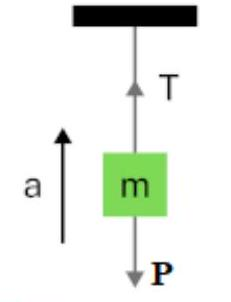
\includegraphics[width=3cm]{Images/2023_11_19_4b5f28cc74af8d9f8b65g-02}
\end{center}

$\mathbf{T}=mg+ma$

\begin{center}
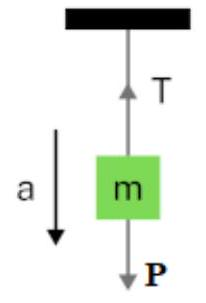
\includegraphics[width=3cm]{Images/2023_11_19_4b5f28cc74af8d9f8b65g-02(2)}
\end{center}

$\mathbf{T}=mg-ma$

\begin{center}
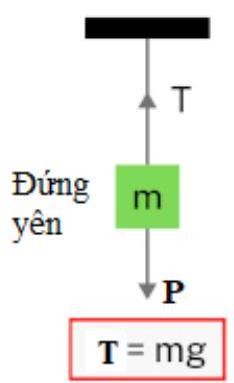
\includegraphics[width=3cm]{Images/2023_11_19_4b5f28cc74af8d9f8b65g-02(3)}
\end{center}

a) $T-P=0 \Rightarrow T=m g=40 \ N$

b) $T-P=m a \Rightarrow T=m g+m a=72 N$

c) $T-P=-m a \Rightarrow T=m g-m a=16 \ N$

}
\haidong{10} \end{vidu}

\begin{vidu}
Một chiếc hộp gỗ được thả trượt không vận tốc ban đầu, từ đầu trên của một tấm gỗ dài $L=2\ m$. Tấm gỗ đặt nghiêng $30^\circ$ so với phương ngang. Hệ số ma sát giữa đáy hộp và mặt gỗ là $0,2$. Lấy $g=9,8\ m/s^2$. Hỏi sau bao lâu thì hộp trượt xuống đến đầu dưới của tấm gỗ.	
\haidong{10}\loigiai{

\immini[thm]{\begin{itemize}
\item Hộp (coi là chất điểm) chịu tác dụng của ba lực: trọng lực $\vec P$, phản lực $\vec N$ và lực ma sát trượt $\vec F_{ms}$ (Hình 20.4a).
\item Phân tích trọng lực $\vec P$ thành hai lực $\vec P_x,\ \vec P_y$ (Hình 20.4b) và áp dụng định luật 2 Newton theo hai trục Ox, Oy:
\begin{align*}
\begin{cases}
&F_x=mg.\sin \alpha=F_{ms}=ma_x=ma \quad (1)\\
&F_y=N-mg\cos\alpha=0 \quad (2)
\end{cases}
\end{align*}
\item $F_{ms}=\mu N$
\item Giải hệ phương trình: $a=g\left(\sin\alpha-\mu \cos\alpha\right)$
\item Thay số ta được: $a=g\left(\sin 30^\circ-0,2\cos 30^\circ\right)\approx 3,2\ m/s^2$
\item Hộp trượt xuống với gia tốc $a=3,2\ m/s^2$, cùng chiều với trục Ox.
\item Áp dụng công thức:  $L=\dfrac{1}{2}at^2\Rightarrow t=\sqrt{\dfrac{2L}{a}}=\sqrt{\dfrac{2.2}{3,2}}\approx 1,1\ s$.
\end{itemize}}{\begin{tikzpicture}[scale=1,thick,>=stealth']
\tkzInit[ymin=-4,ymax=0.5,xmin=-0.5,xmax=5.5]\tkzClip
\begin{scope}[shift={(0,0)},rotate=-30]
\node  at  (2.3,0)  [shape=rectangle,draw=red,pattern=dots,minimum height=0.5cm,minimum width=0.6cm, rounded corners=1pt,rotate=-30]  {};
\draw[very thick,blue,->](2,-0.25)coordinate(o)--++(180:0.5)node[below,black,xshift=-10pt]{$\vec{F}_{ms}$};
\draw[fill=white](2,-0.25)circle(1.2pt);
\draw[very thick,blue,->](2.3,0)--++(0:0.7)node[above,black,xshift=10pt]{$\vec{P}_x$}coordinate(px);
\draw[very thick,blue,->](2.3,0)coordinate(o')--++(90:1.2)node[right,black]{$\vec{N}$};
\draw[very thick,blue,->](2.3,0)--++(-90:1.2)node[left,black]{$\vec{P}_y$}coordinate(n);
\draw[very thick,blue,->](2.3,0)--++(-60:1.4)node[right,black,yshift=5pt]{$\vec{P}$}coordinate(p);
\draw[dashed,thin](px)--(p)--(n);
\draw[fill=white](2.3,0)circle(1.2pt);
\draw(0,-0.27)coordinate(a)--++(0:6)coordinate(b)--++(210:5)coordinate(c);
\fill[pattern=north east lines](b)--(c)--++(300:0.1)--++(390:5);
\tkzMarkAngles[size=0.5cm](a,b,c)
\tkzLabelAngle[pos=-0.8](a,b,c){$\alpha$}
\tkzMarkAngles[size=0.5cm](px,p,o')
\tkzLabelAngle[pos=0.7](px,p,o'){$\alpha$}
\end{scope}
\end{tikzpicture}}
}
\haidong{10} \end{vidu}
\begin{vidu}
\impicinpar{Cho cơ hệ như hình vẽ. Vật $A$ có khối lượng $m_1=200\ g$, vật $B$ có khối lượng $m_2=120\ g$ nối với nhau bởi một sợi dây nhẹ, không dãn. Biết hệ số ma sát trượt giữa hai vật và mặt phẳng ngang là $\mu=0,4$. Tác dụng vào $B$ một lực kéo $F=1,5\ N$ theo phương ngang như hình vẽ. Lấy $g=9,8\ m/s^2$.
\begin{itemize}
\item[a)] Tính gia tốc chuyển động của hệ
\item[b)] Tính độ lớn lực căng dây nối hai vật $A$ và $B$.
\end{itemize}}{	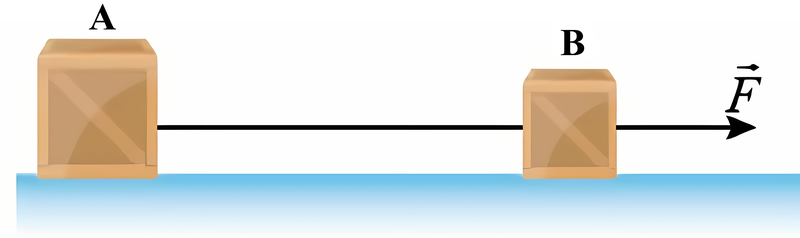
\includegraphics[width=6cm]{Images/2431}} 
\haidong{20}	\loigiai{

Cách 1:

\begin{center}
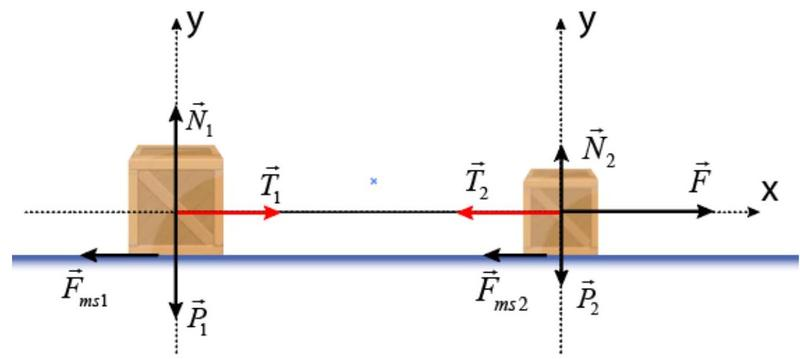
\includegraphics[width=8cm]{Images/2023_11_30_708f45f48fb252b4634cg-05(2)}
\end{center}

Các lực tác dụng lên vật được biểu diễn như hình vẽ.

Xét vật 1:
Coi vật 1 như một chất điểm:
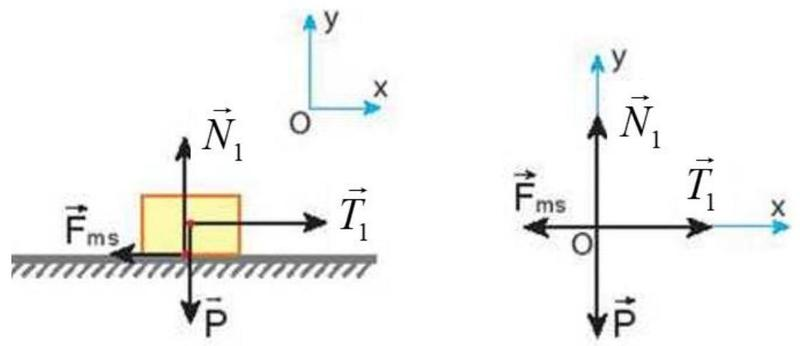
\includegraphics[width=8cm]{Images/2023_11_30_708f45f48fb252b4634cg-06}

Áp dụng định luật II Newton theo các trục $O x$ và $O y$:

Oy: $N_1=P_1=m_1 g$

Mà $F_{m s 1}=\mu \cdot N_1=\mu \cdot m_1 g$

$O x: T_1-F_{m s 1}=m a_1 \Rightarrow T_1-\mu \cdot m_1 g=m_1 \cdot a_1 \Rightarrow T_1=\mu \cdot m_1 g+m_1 \cdot a_1$

Xét vật 2:
$O y: N_2=P_2=m_2 g \Rightarrow F_{m s 2}=\mu N_2=\mu m_2 g$

$O x: F-T_2-F_{m s 2}=m a_2 \Rightarrow T_2=F-\mu m_2 g-m_2 a_2$

Mà sợi dây nhẹ, không dãn nên $T=T_1=T_2$ và $a_1=a_2$.

Suy ra: $\mu \cdot m_1 g+m_1 \cdot a=F-\mu m_2 g-m_2 a$

$\Rightarrow a\left(m_1+m_2\right)=F-\mu g\left(m_2+m_1\right)$

$\Rightarrow a=\dfrac{F}{m_1+m_2}-\mu g=\dfrac{1,5}{0,2+0,12}-0,4.9.8=0,7675\ m/s^2$

$T=T_1=T_2=\mu \cdot m_1 g+m_1 \cdot a=m_1(\mu \cdot g+a)=0,2(0,4.9,8-0,7675)=0,9375 N$

Cách 2:
\begin{center}
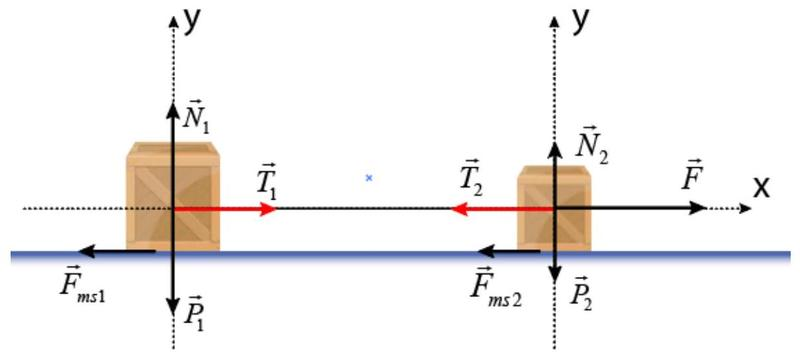
\includegraphics[width=8cm]{Images/2023_11_30_708f45f48fb252b4634cg-06(1)}
\end{center}

Xét 2 vật là một hệ tổng thể.

Áp dụng định luật II Newton cho hệ vật: $\vec{F}+\vec{F}_{m s 1}+\vec{P}_1+\vec{N}_1+\vec{F}_{m s 2}+\vec{P}_2+\vec{N}_2=\left(m_1+m_2\right) \vec{a}(1)$

\begin{itemize}
\item Chọn hệ Oxy như hình vẽ.

\item Chiếu (1)/Oy, ta có: $N_1+N_2=P_1+P_2=g \cdot\left(m_1+m_2\right)$

\item Chiếu (1)/Ox, ta có: $F-F_{m s_1}-F_{m s_2}=\left(m_1+m_2\right) a$

\end{itemize}

$
\begin{aligned}
\Rightarrow a= & \dfrac{F-\mu N_1-\mu N_2}{m_1+m_2} \\
& =\dfrac{F-\mu g\left(m_1+m_2\right)}{m_1+m_2} \\
& =\dfrac{F}{m_1+m_2}-\mu g \\
& =\dfrac{1,5}{0,2+0,12}-0,4.9,8=0,7675\ m/s^2
\end{aligned}
$

b) Lực căng dây $T_1=T_2=T$, áp dụng định luật II Newton cho vật $A: \vec{T}+\vec{P}+\vec{N}+\vec{F}_{m s 1}=m_1 \vec{a}(2)$

Chiếu (2)/Ox, ta có: $T-F_{m s 1}=m_1 a=>T=F_{m s 1}+m_1 a=\mu m_1 g+m_1 a=m_1(\mu g+a)=0,9375 N$

}
\haidong{10} \end{vidu}
%\newpage
\begin{vidu}
\impicinpar{Cho cơ hệ như hình vẽ. Vật thứ nhất có khối lượng $m_1=1\ kg$, vật thứ hai có khối lượng $m_2=3\ kg$ nối với nhau bởi một sợi dây nhẹ, không dãn. Biết hệ số ma sát trượt giữa hai vật và mặt phẳng ngang là $\mu=0,1$. Tác dụng vào vật thứ $2$ một lực kéo $F=5\ N$ theo phương hợp với phương ngang một góc $\alpha=30^\circ$. Lấy $g=9,8\ m/s^2$. Tính gia tốc của mỗi vật và lực căng của dây nối.}{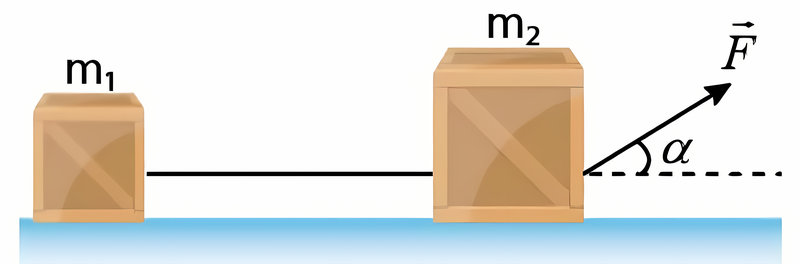
\includegraphics[width=5.25cm]{Images/2432}}
\haidong{15}
\loigiai{
Xét 2 vật là một hệ tổng thể.
\begin{center}
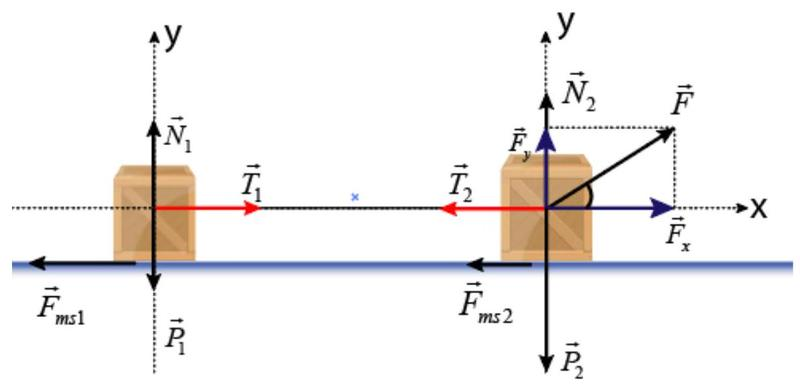
\includegraphics[width=10cm]{Images/2023_11_30_708f45f48fb252b4634cg-09(1)}
\end{center}

Áp dụng định luật II Newton cho hệ vật: $\vec{F}+\vec{F}_{m s 1}+\vec{P}_1+\vec{N}_1+\vec{F}_{m s 2}+\vec{P}_2+\vec{N}_2=\left(m_1+m_2\right) \vec{a}(1)$

\begin{itemize}
\item Chọn trục Oxy như hình vẽ
\end{itemize}

\begin{itemize}
\item Chiếu (1) /Oy: $N_1-P_1+N_2-P_2+F \cdot \sin \alpha=0 \Rightarrow N_1+N_2=P_1+P_2-F \cdot \sin \alpha$
\end{itemize}

+Chiếu (1) /Ox:

$
\begin{aligned}
& F \cdot \cos \alpha-F_{m s 1}-F_{m s 2}=\left(m_1+m_2\right) a \\
& \Rightarrow a=\dfrac{F \cdot \cos \alpha-\mu\left(N_1+N_2\right)}{m_1+m_2}=\dfrac{F \cdot \cos \alpha-\mu\left(P_1+P_2-F \sin \alpha\right)}{m_1+m_2} \\
& \quad=\dfrac{F \cos \alpha-\mu g\left(m_1+m_2\right)+\mu F \sin \alpha}{m_1+m_2}
\end{aligned}
$

$
=0,165\ m/s^2
$

\begin{itemize}
\item Áp dụng định luật II Newton cho vật $m_1$ theo phương Ox: $-F_{m s 1}+T=m_1 a=>T=\mu m_1 g+m_1 a=m_1(\mu g+a)=1,145 N$
\end{itemize}

}
\haidong{10} \end{vidu}
